\documentclass{article}
\usepackage[left=.75in, right=.75in, top=0.5in, bottom=.75in]{geometry}
\usepackage{graphicx}
\usepackage{amsmath}
\usepackage{amssymb}
\usepackage[section]{placeins}
\title{COMP 576 - Fall 2017\\ Assignment 1}

\begin{document}

\maketitle
\pagenumbering{arabic}

\section*{Backpropagation in a Simple Neural Network}

\subsection*{1a) Dataset}

	\begin{figure}[!ht]
		\centering
		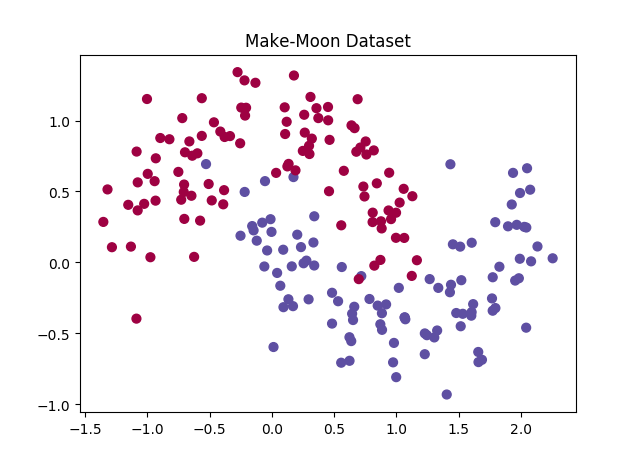
\includegraphics[width=90mm]{figures/makemoondata.png}
		\caption{Make Moon Dataset}
	\end{figure}


\subsection*{1b) Derivatives of Activation Functions}
Sigmoid: 
	\begin{align*}
		f(x) &= \frac{1}{1+e^{-x}} = (1+e^{-x})^{-1}\\ \\
		\frac{d(1+e^{-x})^{-1}}{dx} &= (1+e^{-x})^{-2} (e^{-x})\\\\
		&=\frac{e^{-x}}{(1+e^{-x})^{2}} = \frac{1}{1+e^{-x}}\frac{e^{-x}}{1+e^{-x}}\\\\
		&=\frac{1}{1+e^{-x}}\frac{(1+e^{-x}) - 1}{1+e^{-x}}\\\\
		&= \frac{1}{1+e^{-x}}\left (1 - \frac{ 1}{1+e^{-x}}\right)\\\\
		\boldsymbol{\frac{d(1+e^{-x})^{-1}}{dx}} &\boldsymbol{= f(x)(1-f(x))}\\
	\end{align*}
Tanh:
	\begin{align*}
		f(x) &= \tanh{x} = \frac{\sinh{x}}{\cosh{x}}\\ \\
		\frac{d\left(\frac{\sinh{x}}{\cosh{x}}\right)}{dx}&= \frac{\cosh{x}\cosh{x} - \sinh{x}\sinh{x}}{\cosh^{2}{x}}\\\\
		&= \frac{\cosh^{2}{x}-\sinh^{2}{x}}{\cosh^{2}{x}} = \frac{\cosh^{2}{x}}{\cosh^{2}{x}} -  \frac{\sinh^{2}{x}}{\cosh^{2}{x}}\\\\
		\boldsymbol{\frac{d\left(\frac{\sinh{x}}{\cosh{x}}\right)}{dx}}& \boldsymbol{=1-\tanh^{2}{x}}\\
	\end{align*}
ReLu:
	\begin{equation*}
		f(x) = max(0,x)
	\end{equation*}
\\
	\[
		f(x) = 
			\begin{cases}
				x, & x> 0\\
				0, & \text {otherwise}
			\end{cases}
	\]
\\
	\[
		f'(x) = 
			\begin{cases}
				1, & x> 0\\
				0, & \text {otherwise}
			\end{cases}
	\]

\subsection*{1c) Building the Neural Network}
Three Layer Network
\begin{align}
	z^{1} &= W^{1}x + b^{1}\\
	a^{1} &=actFun(z^{1})\\
	z^{2} &=W^{2}a^{1}+b^{2}\\
	a^{2} &=\hat{y}=softmax(z^{2})
\end{align}
Mean Cross Entropy Loss of Batch
\begin{equation}
	L(y,\hat{y}) = -\frac{1}{N}\sum_{n=1}^{N}\sum_{i=1}^{C}y_{n,i}\log{\hat{y}_{n,i}}
\end{equation}

\subsection*{1d) Backward Pass - Backpropagation}
Gradients: $\frac{\partial L}{\partial W^{2}}$, $\frac{\partial L}{\partial b^{2}}$, $\frac{\partial L}{\partial W^{1}}$, $\frac{\partial L}{\partial b^{1}}$\\ \\
	\begin{align*}
		\frac{\partial L}{\partial W^{2}} &= \frac{\partial L}{\partial \hat{y}}\frac{\partial \hat{y}}{\partial z^{2}}\frac{\partial z^{2}}{\partial W^{2}}\\ \\
		\frac{\partial z^{2}}{\partial W^{2}} &= \frac{\partial (W^{2}a^{2}+b^{2})}{\partial W^{2}}\\ \\
		\boldsymbol{\frac{\partial z^{2}}{\partial W^{2}}}& \boldsymbol{=a^{2}}
	\\
	\\
		\frac{\partial \hat{y_i}}{\partial z_i^{2}} &= \frac{\partial \left(\frac{e^{z_i^2}}{\sum_{j=1}^Ce^{z_j^2}}\right)}{\partial z_i^2}\\ \\
		&  \textbf{if }   j = i\\ \\		
		& = \frac{e^{z_i^2}\sum_{j=1}^Ce^{z_j^2}-e^{z_i^2}e^{z_j^2}}{\left(\sum_{j=1}^Ce^{z_j^2}\right)^2} = \frac{e^{z_i^2}(\sum_{j=1}^Ce^{z_j^2}-e^{z_j^2})}{\sum_{j=1}^Ce^{z_j^2}\sum_{j=1}^Ce^{z_j^2}}\\ \\
		\boldsymbol{\frac{\partial \hat{y_i}}{\partial z_i^{2}}} & \boldsymbol{=\hat{y_i}(1-\hat{y_i})}
	\end{align*}
	\begin{align*}
		&  \textbf{if }   j \neq i\\ \\
		\frac{\partial \hat{y_i}}{\partial z_j^{2}}& = \frac{0-e^{z_i^2}e^{z_j^2}}{(\sum_{j=1}^Ce^{z_j^2})^2} \\\\
		\boldsymbol{\frac{\partial \hat{y_i}}{\partial z_j^{2}}} & \boldsymbol{=-\hat{y_i}\hat{y_j}}
	\\
	\\
		\frac{\partial L}{\partial \hat{y_i}} &= -\frac{1}{N}\sum_{n=1}^N\sum_{i=1}^C\frac{\partial (y_i\log{\hat{y_i}})}{\partial \hat{y_i}} = -\frac{1}{N}\sum_{n=1}^N\sum_{i=1}^C y_i \left(\frac{1}{\hat{y_i}} \right) \frac{\partial \hat{y_i}}			  			{\partial z_i^2}\\ \\
		&  \forall i \\ \\
		&= -\frac{1}{N}\sum_{n=1}^N \left[  \frac{ y_i}{\hat{y_i}} \left(1-\hat{y_i} \right) + \sum_{j\neq i}^C \frac{y_j}{\hat{y_j}}  (-\hat{y_j}\hat{y_i}) \right]\\ \\
		&= -\frac{1}{N}\sum_{n=1}^N \left[ y_i(1-\hat{y_i}) - \sum_{j\neq i}^C y_j\hat{y_i} \right]\\ \\
		&= \frac{1}{N}\sum_{n=1}^N \left[ -y_i+y_i\hat{y_i} +  \sum_{j\neq i}^Cy_j\hat{y_i} \right]\\
		&= \frac{1}{N}\sum_{n=1}^N \left[ -y_i+ \sum_{j= 1}^Cy_j\hat{y_i} \right]\\ \\
		&= \text{since } \boldsymbol{y_j} \text{ is one-hot encoded}\\ \\
		&\implies \sum_{j=1}^Cy_j = 1\\ \\
		\boldsymbol{\therefore{} \frac{\partial L}{\partial z_i^2}} &= \boldsymbol{\frac{1}{N}\sum_{n=1}^N(\hat{y_i}-y_i)}
	\\
	\\
		& \textbf{Let } \delta^3 = (\hat{y_i}-y_i)\\ \\
		\frac{\partial L}{\partial W^2} &= \frac{1}{N}\sum_{n=1}^N\delta^3a^3\\\\
		\boldsymbol{\frac{\partial L}{\partial W^2}}& \boldsymbol{=\frac{1}{N}a^{1T}\delta^3} \\ \\
	\end{align*}
	\begin{align*}
		\frac{\partial L}{\partial b^2} &= \frac{\partial L}{\partial \hat{y}}\frac{\partial \hat{y}}{\partial z^2}\frac{\partial z^2}{\partial b^2}\\ \\
		\frac{\partial z^2}{\partial b^2} &= 1\\\\
		\boldsymbol{\frac{\partial L}{\partial b^2}} & \boldsymbol{=\frac{1}{N}\sum_{n=1}^C\delta^3}
	\\
	\\
		\frac{\partial L}{\partial W^1} &=\underbrace{ \frac{\partial L}{\partial \hat{y}}\frac{\partial \hat{y}}{\partial z^2}}_{\frac{1}{N}\sum_{i=1}^N\delta^3}
			\overbrace{\frac{\partial z^2}{\partial a^1}}^{W^2}
			\underbrace{\frac{\partial a^1}{\partial z^1}}_{f'(z^1)}
			\overbrace{\frac{\partial z^1}{\partial W^1}}^x\\ \\
		&= \frac{1}{N}W^{2T}\delta^3f'(z^1)\\ \\
		& \textbf{Let } \delta^2 = W^{2T}\delta^3f'(z^1)\\ \\
		&= \frac{1}{N}\delta^2x\\ \\
		\boldsymbol{\frac{\partial L}{\partial W^1}} & \boldsymbol{= \frac{1}{N}x^T\delta^2}
	\\
	\\
		\frac{\partial L}{\partial b^1} &= \underbrace{\frac{\partial L}{\partial \hat{y}}
			\frac{\partial \hat{y}}{\partial z^2}
			\frac{\partial z^2}{\partial a^1}
			\frac{\partial a^1}{\partial z^1}}_{\frac{1}{N}\delta^2}
			\overbrace{\frac{\partial z^1}{\partial b^1}}^1\\ \\
		\boldsymbol{\frac{\partial L}{\partial b^1}} &\boldsymbol{= \frac{1}{N}\delta^2}\\ \\
	\end{align*}
	
\subsection*{1e) Training Network}
	\begin{figure}[!htb]
		\centering
		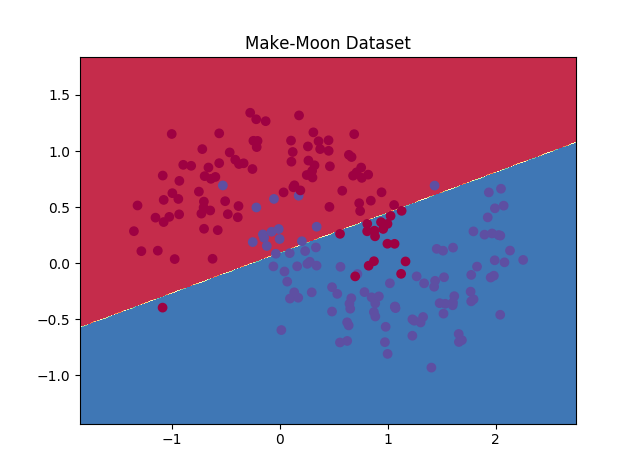
\includegraphics[width=90mm]{figures/sigmoid.png}
		\caption{Trained Network Using Sigmoid Activation Function}
	\end{figure}
	
		\begin{figure}[!htb]
		\centering
		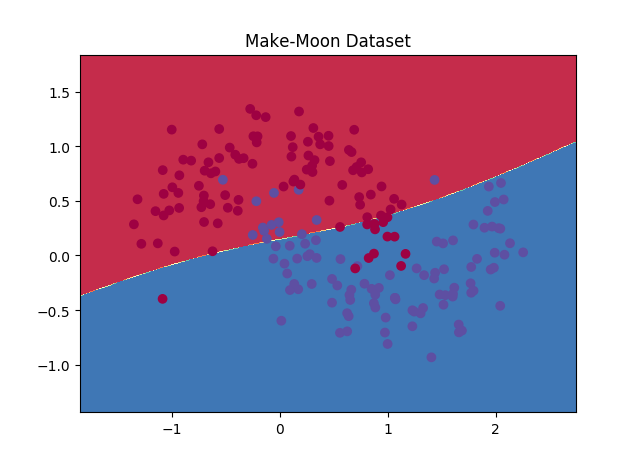
\includegraphics[width=90mm]{figures/tanh.png}
		\caption{Trained Network Using Tanh Activation Function}
	\end{figure}

	\begin{figure}[!htb]
		\centering
		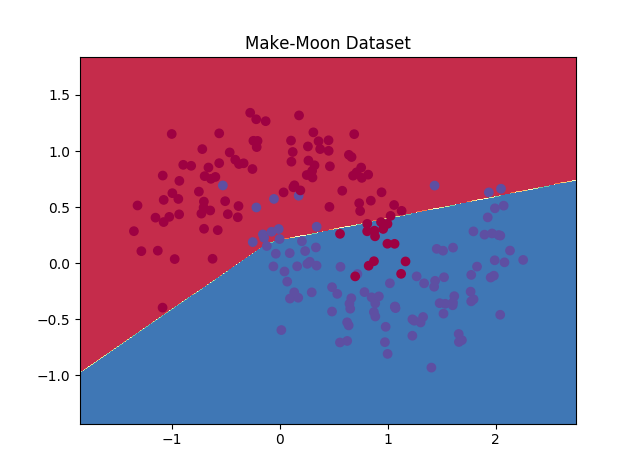
\includegraphics[width=90mm]{figures/relu.png}
		\caption{Trained Network Using ReLu Activation Function}
	\end{figure}

\subsection*{1e.2Using more Hidden Neurons}

	\begin{figure}[ht]
		\centering
		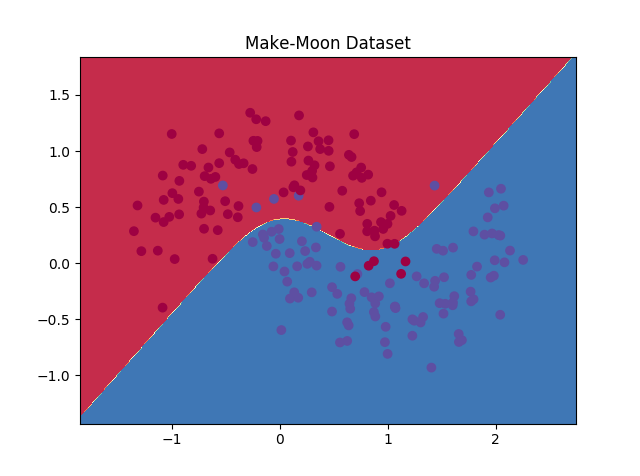
\includegraphics[width=90mm]{figures/tanh_nnh50.png}
		\caption{Trained Network Using Tanh Activation Function and 50 Hidden Neurons}
	\end{figure}
	
		\begin{figure}[!htbp]
		\centering
		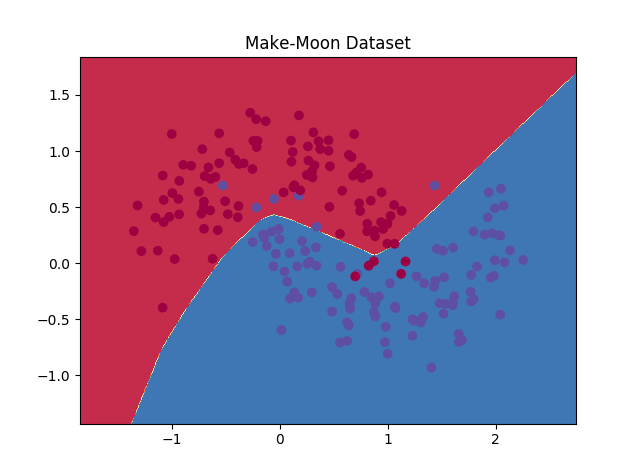
\includegraphics[width=90mm]{figures/relu_nnh50.png}
		\caption{Trained Network Using ReLu Activation Function and 50 Hidden Neurons}
	\end{figure}
	
	Incresing the number of neurons makes it have more degrees of freedome.
	
\end{document}